% Extracted from chainRule.tex, problem #3
\begin{problem}
  Given the following graphs of $f$ and $g$ (both piecewise
  linear functions), define new functions $u(x) = f(g(x))$ and
  $v(x) = f(x)g(x)$.  Find:

% image replaced with tikzpic below
%  \begin{image}[0.4\linewidth]
%    \includegraphics[trim= 170 420 250 230]{Figure7.pdf}
%  \end{image}

	  \begin{center}
		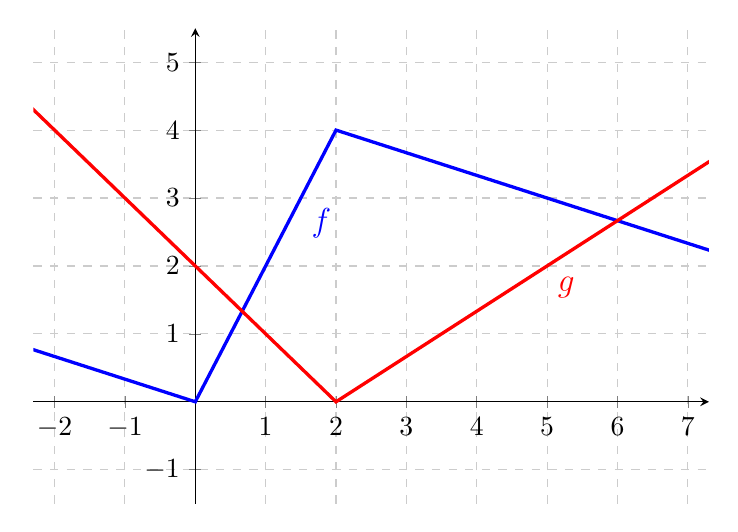
\begin{tikzpicture}
			\begin{axis}[
				xmin=-2.3, xmax=7.3, ymin=-1.5,ymax=5.5,    
				axis lines =middle, 
				every axis y label/.style={at=(current axis.above origin),anchor=south},
				every axis x label/.style={at=(current axis.right of origin),anchor=west},
				xtick={-2,...,7}, ytick={-1,...,5},
				grid=major, width=4in, height = 3in,
				grid style={dashed, gray!40}
				]
				\path[draw, color=blue, very thick] (axis cs:-3,1) --  (axis cs:0,0) -- (axis cs:2,4) node[pos=0.75, below right]{\large{$f$}}  -- (axis cs: 8,2);
				\path[draw, color=red, very thick] (axis cs:-3,5) --  (axis cs:2,0) -- (axis cs:8,4) node[pos=0.5, below right]{\large{$g$}};	
			\end{axis}
		\end{tikzpicture}
	\end{center}


  \begin{enumerate}	
  \item $u'(1)$
\WkstHop
	\begin{freeResponse}
      $u'(x) = \ddx(f(g(x))) = f'(g(x)) \cdot g'(x)$.  So,
      \begin{align*}
        u'(1) &= f'(g(1)) \cdot g'(1) \\
              &= f'(1) \cdot (-1) \\
              &= (2)(-1) = -2 
      \end{align*}  
    \end{freeResponse}
		
		
		
	
  \item $v'(1)$
\WkstHop
	\begin{freeResponse}
      $v'(x) = \ddx(f(x)g(x)) = f'(x)g(x) + f(x)g'(x)$.  So,
      \begin{align*}
        v'(1) &= f'(1) g(1) + f(1) g'(1) \\
              &= (2)(1) + (2)(-1) \\
              &= 0
      \end{align*}
    \end{freeResponse}

  \item $\displaystyle \lim_{x\to 1} \dfrac{\sqrt{g(x)}-1}{x-1}$
\WkstHop
	\begin{freeResponse}
	This is asking for $\eval{\ddx( \sqrt{g(x)} )}_{x=1}$. 
	By the Chain Rule, $\ddx( \sqrt{g(x)} ) = \dfrac{g'(x)}{2\sqrt{g(x)}}$ so 
	\begin{align*}
		\eval{\ddx( \sqrt{g(x)} )}_{x=1} &= \dfrac{g'(1)}{2\sqrt{g(1)}}\\
			&= \dfrac{-1}{2\sqrt{1}}\\
			&= -\dfrac{1}{2}.
	\end{align*}
    \end{freeResponse}
  \end{enumerate}		
			
	
		
\end{problem}
